%!TEX root = ../thesis.tex
%*******************************************************************************
%****************************** Third Chapter **********************************
%*******************************************************************************
\chapter{Evaluation}

% **************************** Define Graphics Path **************************
\ifpdf
    \graphicspath{{07_Chapter6/Figs/Raster/}{07_Chapter6/Figs/PDF/}{07_Chapter6/Figs/}}
\else
    \graphicspath{{07_Chapter6/Figs/Vector/}{07_Chapter6/Figs/}}
\fi

\section{Evaluation Settings}

Appendix A presents a list of synthetic functions and real datasets that are used to evaluate the effectiveness of a Bayesian Optimization algorithm. 
I conduct experiments in the following settings as mentioned in chapter \ref{syntheticFunction}.
Furthermore, we will shortly discuss the underlying real dataset, which is hyper-parameter-configurations from the SwissFEL x-ray laser.

\section{Quantitative evaluation}
To recapitulate, I will use log-likelihood measures and cumulative regret to compare the performance of different algorithms.


\section{Qualitative evaluation}

\subsection{Feature selection}
The goal of this task is to see, if the revised active subspace identification algorithms can effectively do feature selection.
For this task, I set up a function $ f $ that looks as follows:

\def\B{
\begin{bmatrix}
    (x - a_0)^2 \\
    (y - a_1)^2
\end{bmatrix}}

\begin{equation} \label{eq:FeatureExtension}
f \left( W \B \right) \approx g \left( x \right)
\end{equation} 

where $x_0, x_1$ are constants. \\

For this specific experiment, the function $f$ is chosen to be a one-dimensional parabola. 
As such, $W$ is chosen as a matrix on the Stiefel manifold with dimensions $\mathbf{R}^{d \times D}$

Doing a feature extension over $x$ and $y$, we can get the following feature representation:

\def\PHI{
\begin{bmatrix}
	x_0^2 \\
	x_1^2 \\
	x_0 \\
	x_1 \\
    1
\end{bmatrix}}


\def\WtoPhi{
\begin{bmatrix}
	w_0 \\
    w_1 \\
	-2 w_0 a_0 \\
	-2 w_1 a_1 \\
	w_0 a_0^2 + w_1 a_1^2
\end{bmatrix}}

\begin{figure}[h]

\begin {minipage}{0.47\textwidth}
  \centering
  \begin{equation}
    \PHI
  \end{equation}
  \caption{Polynomial Kernel applied to vector $[x_0, x_1]$}
\end{minipage}
\hfill
\begin {minipage}{0.47\textwidth}
  \centering
  \begin{equation}
    \WtoPhi
  \end{equation}
  \caption{Corresponding weight matrix equivalent to \ref{eq:FeatureExtension} when applied on a parabola}
\end{minipage}

\end{figure}

To run experiments, I instantiate the "real" matrix, which should be found by the algorithm with the values $w_0 = 0.589$, $w_1 = 0.808$ (randomly sampled as a matrix on the Stiefel manifold), $a_0 = -0.1$, $a_1 = 0.1$ (chosen by me as coefficients). \\

I apply the algorithm 1. from \citep{Tripathy} to identify the active projection matrix.
The optimization algorithm has 50 samples to discover the hidden matrix, which it seemingly does up do a certain degree of accuracy.
Similar results are achieved for repeated tries.
The following figure shows the real matrix, and the matrix the algorithm has found.

\def\realW{
\begin{bmatrix}
	0.589 \\
    0.808 \\
	0.118 \\
	-0.162 \\
	0.823
\end{bmatrix}}

\def\okW1{
\begin{bmatrix}
	-0.355 \\
    	-0.533 \\
    	-0.908 \\
    	0.099 \\
    -0.756 
\end{bmatrix}}

\begin{figure}[h] 
\begin {minipage}{0.47\textwidth}
  \centering
  \begin{equation} \label{fig:realMatrix}
    \realW
  \end{equation}
  \caption{Real matrix}
\end{minipage}
\hfill
\begin {minipage}{0.47\textwidth}
  \centering
  \begin{equation} \label{fig:foundMatrix}
    \okW1
  \end{equation}
  \caption{Matrix found by optimization algorithm}
\end{minipage}
\end{figure}

Although one can see that the element wise difference between the two matrices \ref{fig:realMatrix} and \ref{fig:foundMatrix} are high (between $0.05$ and $0.15$), one can see that the matrix recovery is successful in finding an approximate structure that resembles the original structure of the features.
One should observe that the found matrix is an approximate solution to the real matrix in the projection. I.e. the matrix found is close to the real matrix, but multiplied by $-1$. \\

Because in this case, I applied the feature selection algorithm on a vector-matrix (only one column), one can quantify the reconstruction of the real matrix through the found matrix by the normalized scalar product.
This quantity is a metric between $0$ and $1$, where $0$ means that both vectors are orthogonal, and $1$ means that both vectors overlap.

\begin{equation}
\text{overlap}(u, v) = \frac{| \langle u, v \rangle |}{\langle u, u \rangle}
\end{equation}
where $u$ is the real vector, and $v$ is the found vector.

Inserting the actual values into the field, we get $0.79$, which is a good value for the feature vector found, and the trained number of datapoints which is 50. \\
 
 This experiment shows that algorithm 1. from \citep{Tripathy} successfully allows a viable option to other feature selection algorithms, by providing a measure, where the optimal linear projection is found. 
 However, one must notice that other feature selection algorithms (such as SVM), are more efficient, and will provide better results with higher probability if applied on a similar kernel. \\
 
 One major observation I made was the the increase in the log likelihood of the data w.r.t. the projection matrix did not correlate with the decrease in the angle between the real vs the found projection matrix.
 Also, most often, the angle was at around 40 degrees, which means that only slight improvements over a fully random embedding were made.


\subsection{Subspace identification}
One of the main reasons to use our method is because we allow for subspace identification.
We have the following functions:

\begin{enumerate}
\item 1D Parabola embedded in a 2D space
\item 2D Camelback embedded in a 5D space
\item 2D Sinusoidal and Exponential function embedded in a 5D space
\end{enumerate} //

To be able to visualize the points, I proceed with the following procedure:

I generate testing points (points to be visualized) within the 2D-space in a uniform grid.
I then project these testing points to the dimension of the original function ($2d$ for parabola, else $5d$).
I then let each algorithm learn and predict the projection matrix and GP mean predictions.
If because the transformation from $2D$ space, to $5D$ space and to GP mean prediction is each bijective, we can visualize the $2D$ points with the GP mean prediction right away.
As such, the dimension of the embedding learned does not have impact on the visualization!

In the following figures, blue point shows the sampled real function value.
Orange points shows the sampled mean prediction of the trained GP.
The GPs were each trained on 100 datapoints. 
The points shown below were not used for training at any point, as these are included in the test-set.

% PARABOLA FUNCTION
\begin{figure}[H]
    \centering
    \begin{subfigure}[b]{0.30\textwidth}
        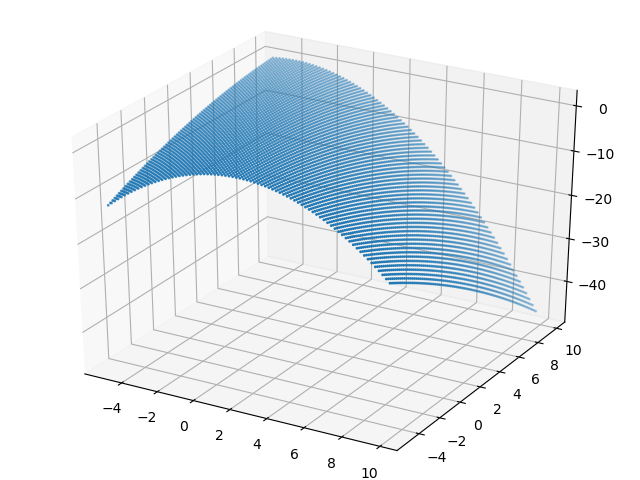
\includegraphics[width=\textwidth]{orig/Parabola-2D->1D.png}
        \caption{Parabola Original}
        \label{fig:gull}
    \end{subfigure}
    %add desired spacing between images, e. g. ~, \quad, \qquad, \hfill etc. 
      %(or a blank line to force the subfigure onto a new line)
    \begin{subfigure}[b]{0.30\textwidth}
        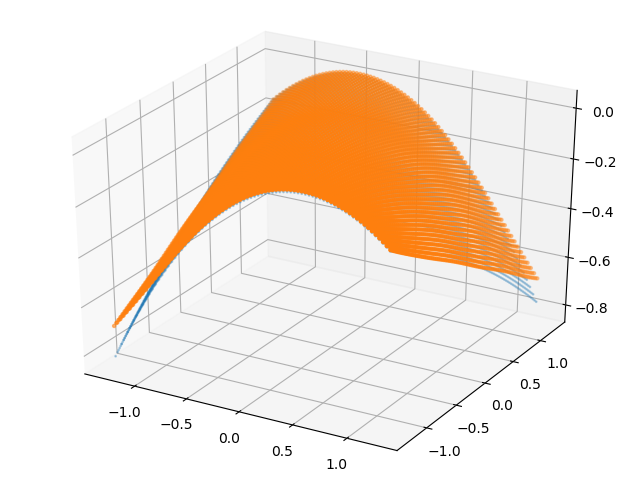
\includegraphics[width=\textwidth]{orig/Parabola-2D->1D_BORING.png}
        \caption{Parabolanusoidal Boring}
        \label{fig:tiger}
    \end{subfigure}
     %add desired spacing between images, e. g. ~, \quad, \qquad, \hfill etc. 
    %(or a blank line to force the subfigure onto a new line)
    \vskip\baselineskip
    \begin{subfigure}[b]{0.30\textwidth}
        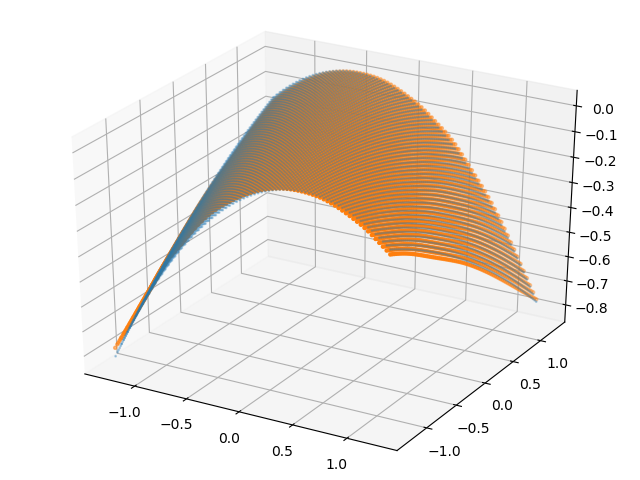
\includegraphics[width=\textwidth]{orig/Parabola-2D->1D_TRIPATHY.png}
        \caption{Parabola Tripathy}
        \label{fig:mouse}
    \end{subfigure}
            %add desired spacing between images, e. g. ~, \quad, \qquad, \hfill etc. 
    %(or a blank line to force the subfigure onto a new line)
    \begin{subfigure}[b]{0.30\textwidth}
        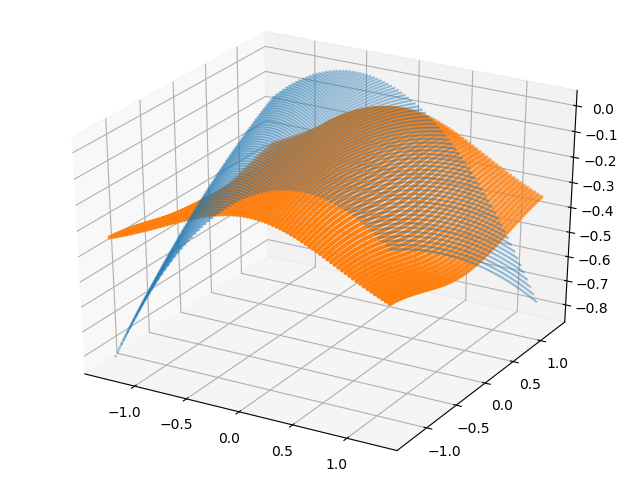
\includegraphics[width=\textwidth]{orig/Parabola-2D->1D_REMBO.png}
        \caption{Parabola Rembo}
        \label{fig:mouse}
    \end{subfigure}
    \caption{Top-Left: The 1D Parabola which is embedded in a 2D space.}\label{fig:animals}
\end{figure}

I set the number of restarts to $14$ and number of randomly sampled datapoints to 100.
Notice that the Tripathy approximation is slightly more accurate than the BORING approximation. 
This is because one of Tripathy's initial starting points were selected better, such that algorithm 3 ran many times before the relative loss terminated the algorithm.
The active subspace projection matrix is of size $\mathbf{R}^{1 \times 2}$

% SINUSOIDAL FUNCTION
\begin{figure}[H]
    \centering
    \begin{subfigure}[b]{0.3\textwidth}
        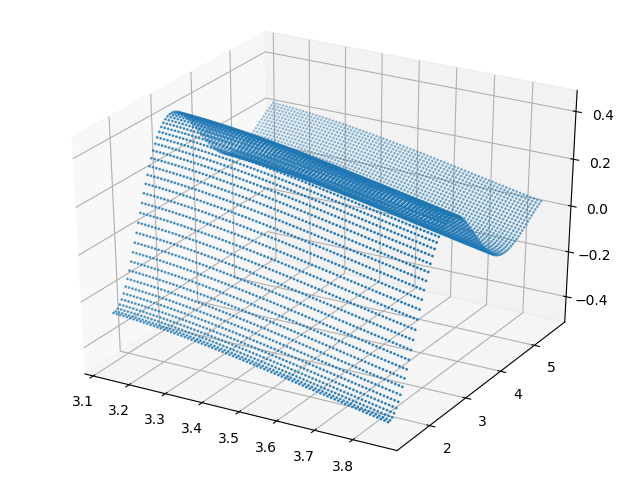
\includegraphics[width=\textwidth]{orig/Sinusoidal-5D->2D.png}
        \caption{Sinusoidal Original}
        \label{fig:gull}
    \end{subfigure}
    ~ %add desired spacing between images, e. g. ~, \quad, \qquad, \hfill etc. 
      %(or a blank line to force the subfigure onto a new line)
    \begin{subfigure}[b]{0.3\textwidth}
        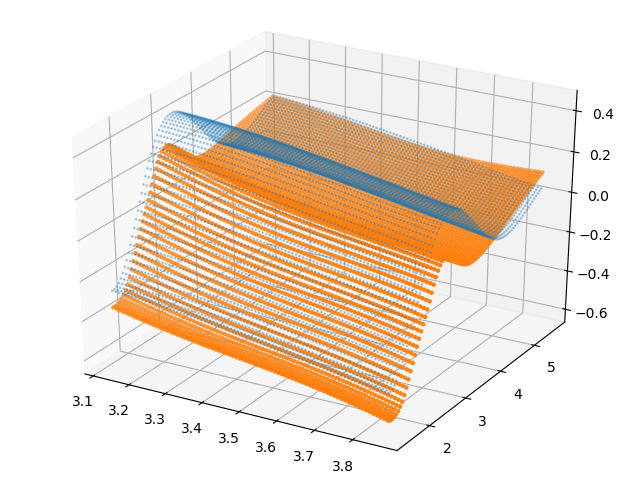
\includegraphics[width=\textwidth]{orig/Sinusoidal-5D->2D_BORING.png}
        \caption{Sinusoidal Boring}
        \label{fig:tiger}
    \end{subfigure}
        \vskip\baselineskip
 %add desired spacing between images, e. g. ~, \quad, \qquad, \hfill etc. 
    %(or a blank line to force the subfigure onto a new line)
    \begin{subfigure}[b]{0.3\textwidth}
        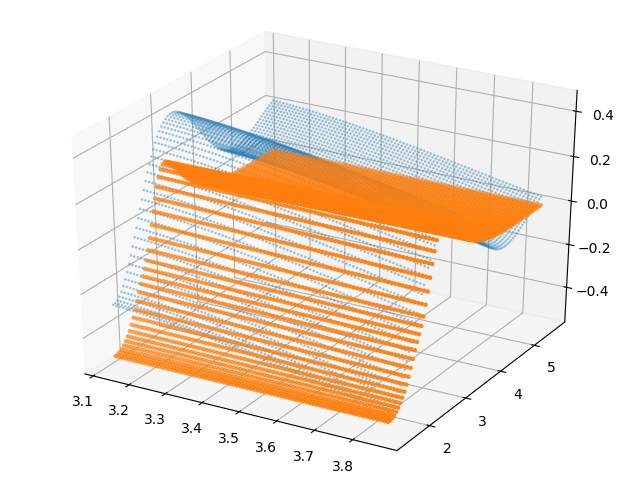
\includegraphics[width=\textwidth]{orig/Sinusoidal-5D->2D_TRIPATHY.png}
        \caption{Sinusoidal Tripathy}
        \label{fig:mouse}
    \end{subfigure}
        ~ %add desired spacing between images, e. g. ~, \quad, \qquad, \hfill etc. 
    %(or a blank line to force the subfigure onto a new line)
    \begin{subfigure}[b]{0.3\textwidth}
        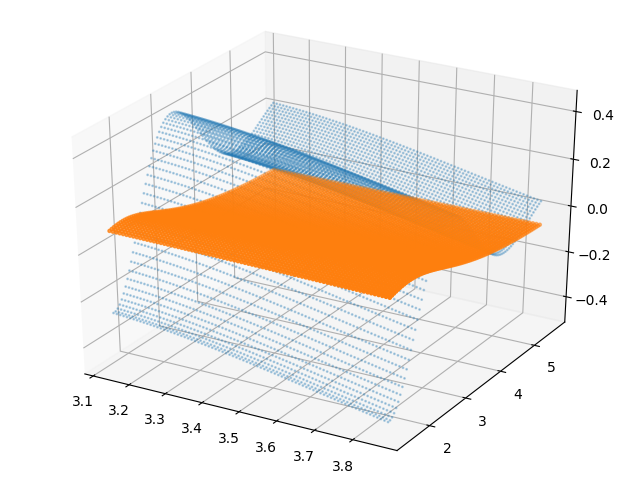
\includegraphics[width=\textwidth]{orig/Sinusoidal-5D->2D_REMBO.png}
        \caption{Sinusoidal Rembo}
        \label{fig:mouse}
    \end{subfigure}
    \caption{Top-Left: The 2D Sinusoidal-Exponential Function which is embedded in a 5D space.}\label{fig:animals}
\end{figure}

I set the number of restarts to $28$ and number of randomly sampled datapoints to 100.
The active subspace projection matrix is of size $\mathbf{R}^{1\times 5}$, as this is a function that exhibits a strong principal component, but that still attains small perturbations among a different dimension.
One can see very well here, that BORING is able to take into account the small perturbations, at a considerably lower cost than Tripathy would be able to.
REMBO ???

% CAMELBACK FUNCTION
\begin{figure}[H]
    \centering
    \begin{subfigure}[b]{0.3\textwidth}
        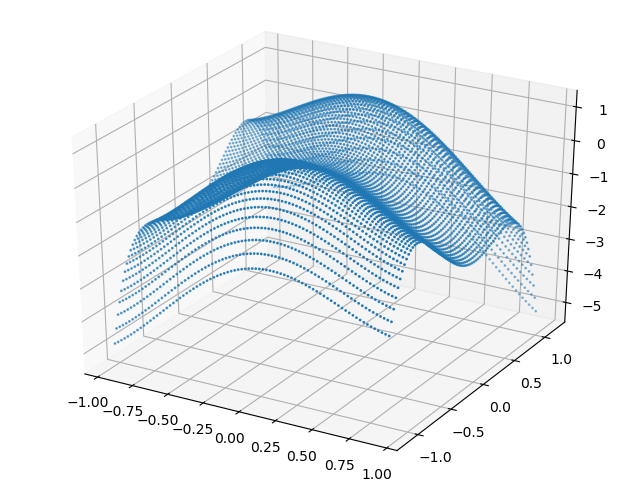
\includegraphics[width=\textwidth]{orig/Camelback-5D->2D.png}
        \caption{Camelback Original}
        \label{fig:gull}
    \end{subfigure}
    ~ %add desired spacing between images, e. g. ~, \quad, \qquad, \hfill etc. 
      %(or a blank line to force the subfigure onto a new line)
    \begin{subfigure}[b]{0.3\textwidth}
        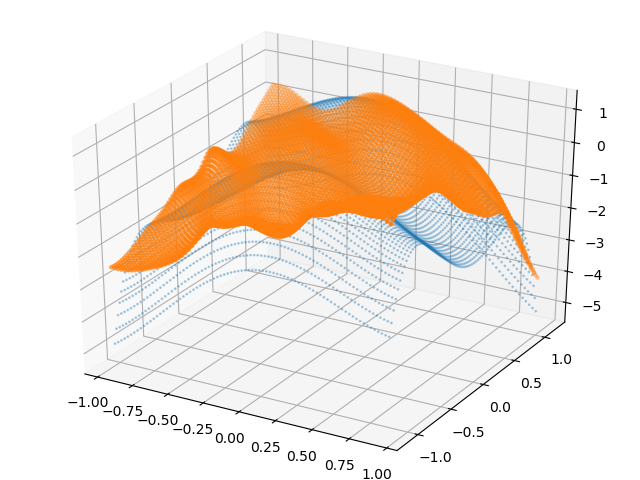
\includegraphics[width=\textwidth]{orig/Camelback-5D->2D_BORING.png}
        \caption{Camelback Boring}
        \label{fig:tiger}
    \end{subfigure}
        \vskip\baselineskip
 %add desired spacing between images, e. g. ~, \quad, \qquad, \hfill etc. 
    %(or a blank line to force the subfigure onto a new line)
    \begin{subfigure}[b]{0.3\textwidth}
        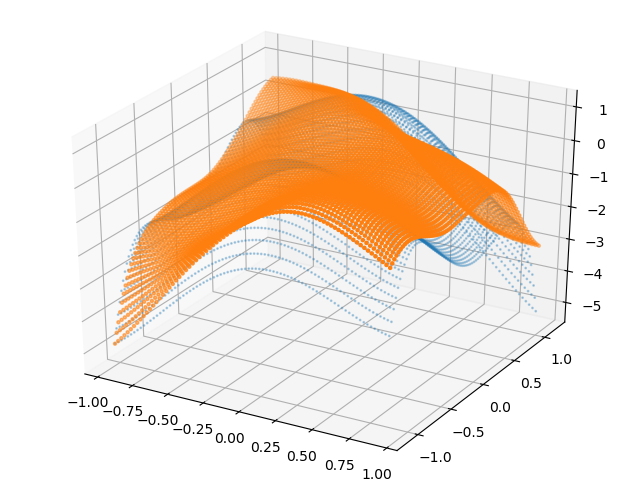
\includegraphics[width=\textwidth]{orig/Camelback-5D->2D_TRIPATHY.png}
        \caption{Camelback Tripathy}
        \label{fig:mouse}
    \end{subfigure}
        ~ %add desired spacing between images, e. g. ~, \quad, \qquad, \hfill etc. 
    %(or a blank line to force the subfigure onto a new line)
    \begin{subfigure}[b]{0.3\textwidth}
        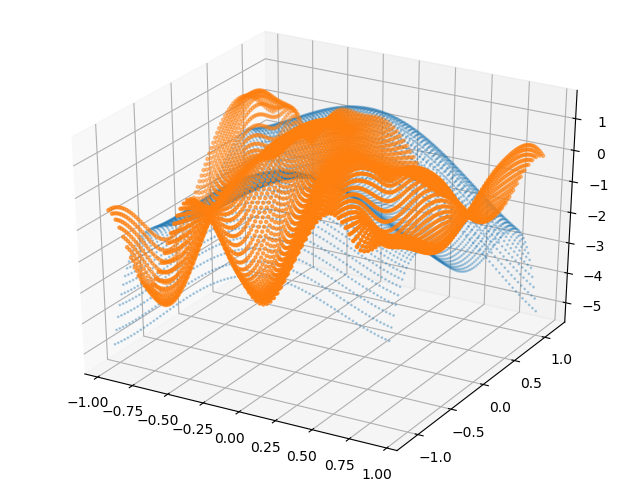
\includegraphics[width=\textwidth]{orig/Camelback-5D->2D_REMBO.png}
        \caption{Camelback Rembo}
        \label{fig:mouse}
    \end{subfigure}
    \caption{Top-Left: The 2D Camelback Function which is embedded in a 5D space.}\label{fig:animals}
\end{figure}

I set the number of restarts to $28$ and number of randomly sampled datapoints to 100.
The active subspace projection matrix is of size $\mathbf{R}^{2 \times 5}$, as this is a function that lives in a 2D space, and has two strong principal components.
Notice that Tripathy and BORING use the exact same algorithm, as the visualization does not allow to add a third axis. 
In other words, BORING does not add any additional orthogonal vector to the model.
As such, it does not add any additional kernels to the model aswell, and is equivalent to tripathy.
REMBO ???

% CAMELBACK 1D PROJECTION
\begin{figure}[H]
    \centering
    \begin{subfigure}[b]{0.3\textwidth}
        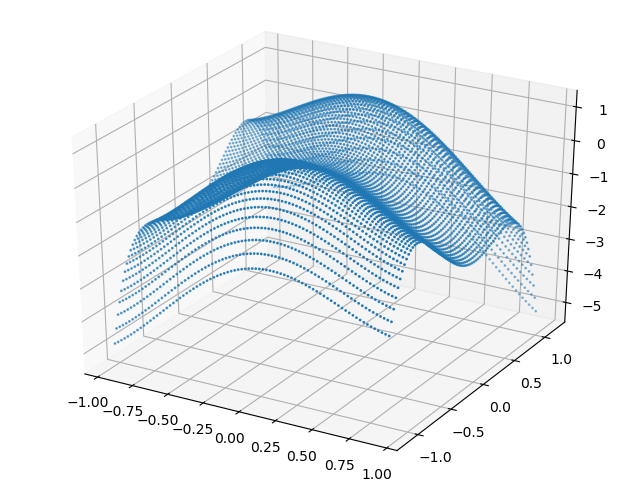
\includegraphics[width=\textwidth]{orig/Camelback-5D->2D.png}
        \caption{Camelback Original}
        \label{fig:gull}
    \end{subfigure}
    ~ %add desired spacing between images, e. g. ~, \quad, \qquad, \hfill etc. 
      %(or a blank line to force the subfigure onto a new line)
    \begin{subfigure}[b]{0.3\textwidth}
        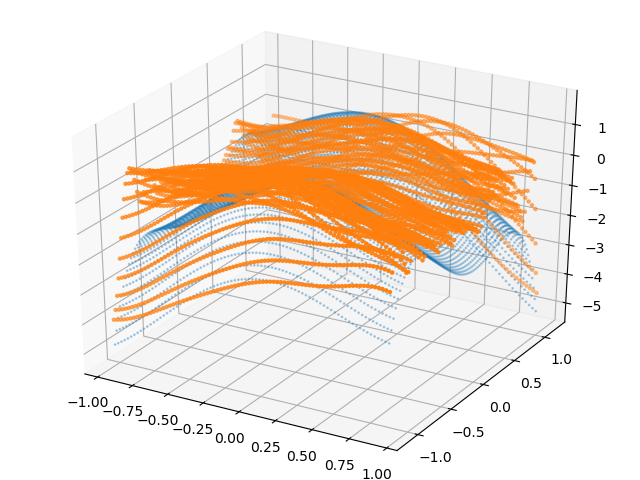
\includegraphics[width=\textwidth]{orig/Camelback-5D->2D_BORING_1D.png}
        \caption{Camelback Boring}
        \label{fig:tiger}
    \end{subfigure}
        \vskip\baselineskip
 %add desired spacing between images, e. g. ~, \quad, \qquad, \hfill etc. 
    %(or a blank line to force the subfigure onto a new line)
    \begin{subfigure}[b]{0.3\textwidth}
        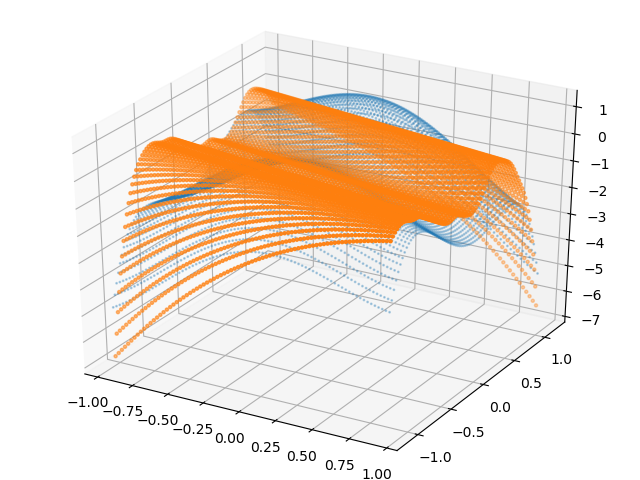
\includegraphics[width=\textwidth]{orig/Camelback-5D->2D_TRIPATHY_1D.png}
        \caption{Camelback Tripathy}
        \label{fig:mouse}
    \end{subfigure}
        ~ %add desired spacing between images, e. g. ~, \quad, \qquad, \hfill etc. 
    %(or a blank line to force the subfigure onto a new line)
    \begin{subfigure}[b]{0.3\textwidth}
        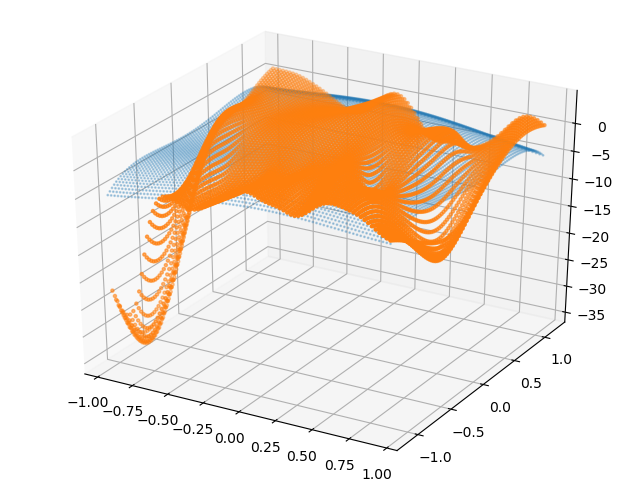
\includegraphics[width=\textwidth]{orig/Camelback-5D->2D_REMBO_1D.png}
        \caption{Camelback Rembo}
        \label{fig:mouse}
    \end{subfigure}
    \caption{Top-Left: The 2D Camelback Function which is embedded in a 5D space.}\label{fig:animals}
\end{figure}

I set the number of restarts to $28$ and number of randomly sampled datapoints to 100.
The active subspace projection matrix is of size $\mathbf{R}^{1 \times 5}$, as I want to explore to what extent complicated functions are explored, when we set the effective dimension lower than the real number of active dimensions.
One can see that tripathy has a much smoother function surface, and that BORING allows to take into consideration smaller local perturbations, as it includes a third random axis.
Whichever is better depends on the application, and BORGIN will be able to adapt better to more points, whereas Tripathy will project multiple points onto the same space.
One can see very well here, that BORING is able to take into account the small perturbations, at a considerably lower cost than Tripathy would be able to.
REMBO ??? 
